%% Supplementary Information, compiled separately from main.tex.
\documentclass[pdflatex,sn-nature]{sn-jnl}

\usepackage{graphicx}
\usepackage{amsmath,amssymb,amsfonts}
\usepackage{booktabs}
\usepackage{textcomp}
\usepackage{url}
\usepackage{xr}
\externaldocument{main}

\graphicspath{{figures/}}

\renewcommand{\thefigure}{S\arabic{figure}}
\renewcommand{\thetable}{S\arabic{table}}

\begin{document}

\title[Supplementary information]{Supplementary information for: A gas-transport model predicts the \textit{Arabidopsis} spaceflight transcriptome, and hardware ventilation resolves true microgravity responses from sealed canister artifacts}

\author*[1]{\fnm{Richard} \sur{Barker}}\email{dr.richard.barker@gmail.com}
\affil[1]{\orgname{Department of Botany, University of Wisconsin-Madison}, \city{Madison}, \state{WI}, \country{USA}}

\maketitle

\section*{Supplementary Figures and Tables}

\begin{figure}[htbp]\centering
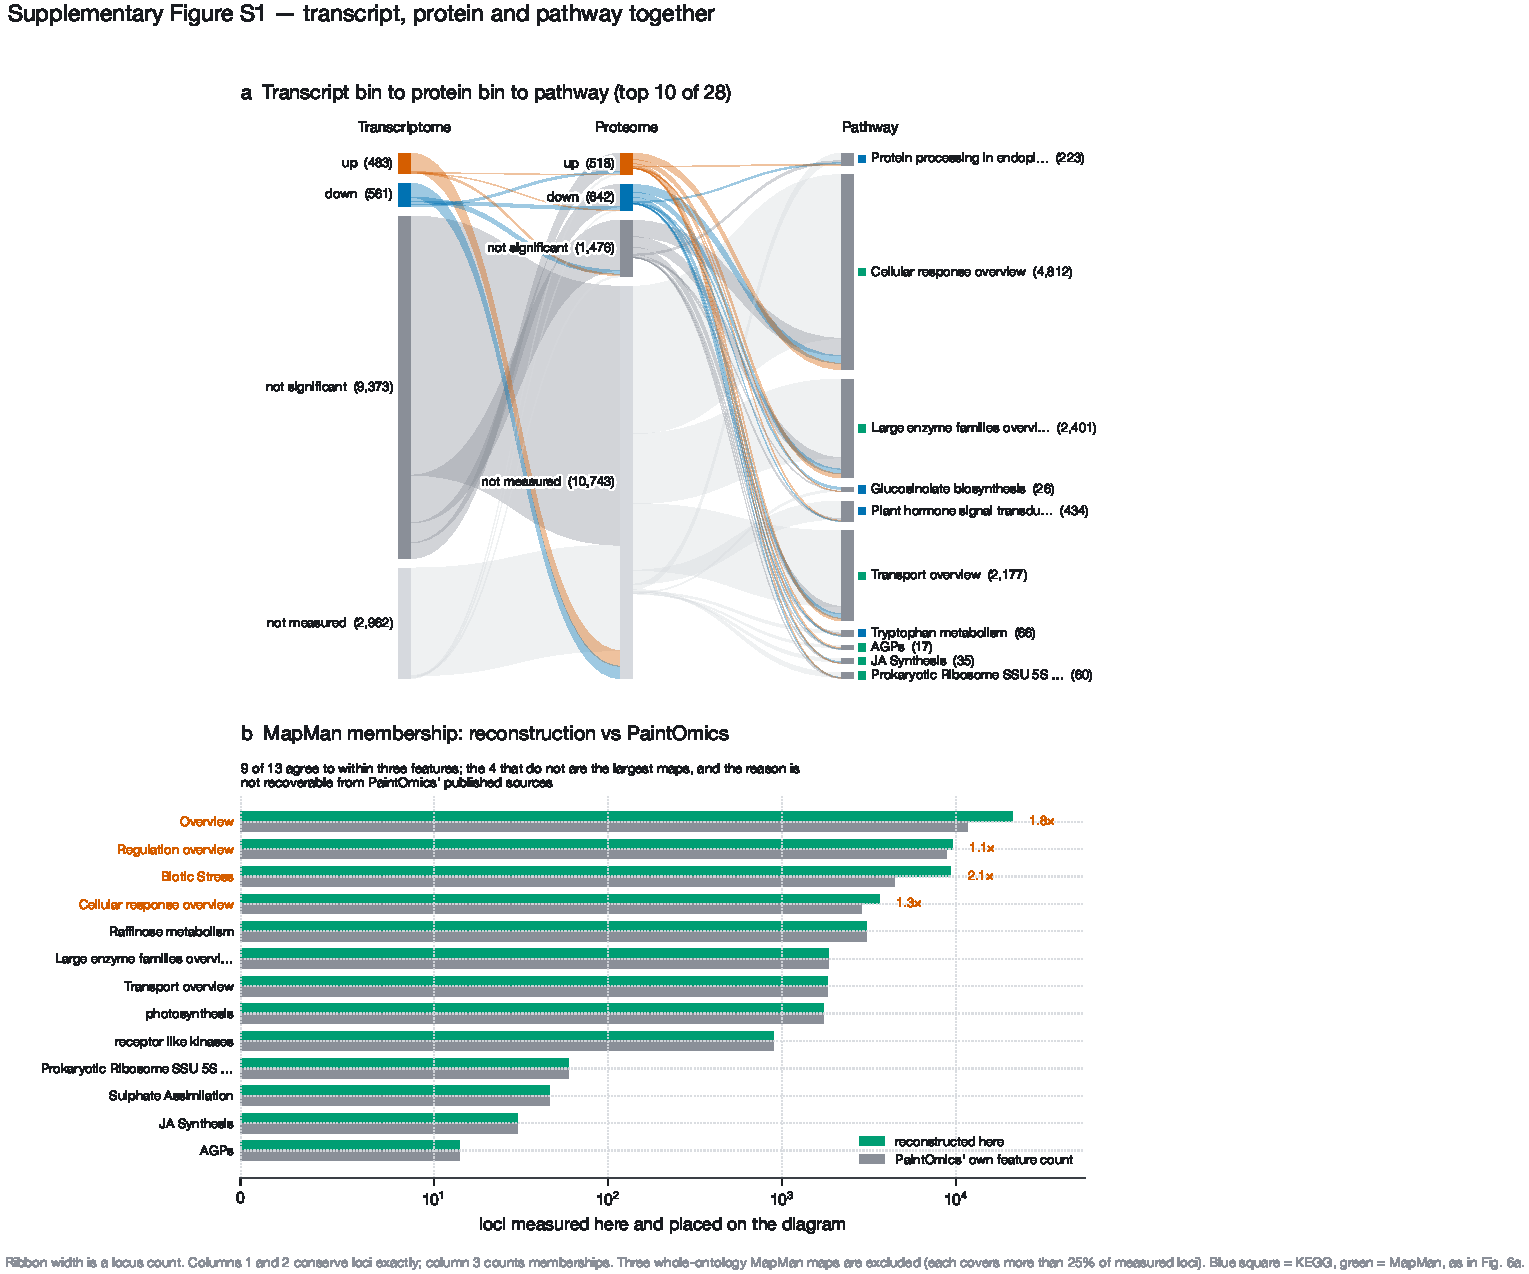
\includegraphics[width=\textwidth]{figS1_sankey.pdf}
\caption{\textbf{Locus-level multi-omics flow and MapMan ontology reconstruction.}
\textbf{a}, Each locus in at least one of the 28 non-whole-ontology significant pathways is placed in one transcript bin and one protein bin, and then into the pathways it belongs to. Ribbon width is proportional to locus count. The pathway column draws the ten most significant pathways; a square gives each pathway's database in the colours of Fig.~\ref{fig:paintomics}a.
\textbf{b}, Reconstructed MapMan diagram membership compared against the feature count PaintOmics reported for each diagram (log scale). Nine of the thirteen diagrams agree to within three features.}
\label{fig:sankey}\end{figure}

\begin{table}[htbp]
\caption{Cross-hardware pathway classification: comparison of the key pathways enriched in sealed BRIC-LED (OSD-522) against ventilated ABRS (OSD-7).}
\label{tab:s1_comparison}
\centering
\fontsize{7.5}{9.5}\selectfont
\setlength{\tabcolsep}{3pt}
\begin{tabular}{lp{3.6cm}rrlp{3.8cm}}
\toprule
DB & Pathway & BRIC-LED $p$ & ABRS $p$ & ABRS Dir & Classification \\
\midrule
K & Protein processing in ER & $8.65\times10^{-9}$ & 0.9456 & Flat & Hardware artifact (volatiles / CO$_2$) \\
M & Cellular response overview & $2.33\times10^{-6}$ & 0.6111 & Down & Hardware artifact \\
M & Biotic Stress & $2.10\times10^{-4}$ & 0.0151 & Up & \textbf{Conserved microgravity response} \\
K & Glucosinolate biosynthesis & $6.02\times10^{-4}$ & 0.8453 & Up & Hardware artifact \\
K & Plant hormone signal transduction & 0.0011 & 0.0516 & Up & Borderline conserved \\
K & Photosynthesis & 0.0080 & 0.8512 & Down & Hardware-modulated \\
K & MAPK signaling pathway & 0.0094 & 0.2322 & Up & Hardware-modulated \\
K & Starch and sucrose metabolism & 0.0186 & 0.5428 & Down & Hardware-modulated \\
K & Photosynthesis - antenna proteins & 0.0217 & 1.0000 & Down & Hardware-modulated \\
M & Raffinose metabolism & 0.0274 & 0.0081 & Up & \textbf{Conserved microgravity response} \\
K & Carbon fixation by Calvin cycle & 0.1420 & 0.0074 & Up & ABRS-specific (CO$_2$ saturated) \\
K & Cysteine and methionine metabolism & 0.2110 & 0.0015 & Down & ABRS-specific \\
\botrule
\end{tabular}
\end{table}

\end{document}
